% =====================================================================
%  Fiche d’activités : les 4 activités du chapitre 3 (physique) sur deux pages A4
%  (activités 1 et 2 page 1, activités 3 et 4 page 2)
%  Travail et énergie cinétique
%  (sans situation de départ, sans zone de nom, sans bandeau de titre)
%  À coller dans le cahier. Compilation : xelatex fiche_unique.tex (deux passes)
%  Le doc 8 est à l’échelle 1 : imprimer à 100 % (sans ajustement à la page).
% =====================================================================
\documentclass[10pt,a4paper]{article}
\usepackage[a4paper,top=.75cm,bottom=.6cm,left=.8cm,right=.8cm]{geometry}
\usepackage{fontspec}
\usepackage{polyglossia}
\setmainlanguage{french}
\usepackage{amsmath}
\usepackage{unicode-math}
\setmainfont{TeX Gyre Pagella}
\setsansfont{Poppins}[Path=fonts/, Extension=.ttf, UprightFont=*-Regular, BoldFont=*-Bold, ItalicFont=*-Italic, BoldItalicFont=*-BoldItalic]
\setmathfont{Latin Modern Math}
\setmathfont[range={it/{latin,Latin,greek,Greek}}]{texgyrepagella-italic.otf}
\setmathfont[range={up/{latin,Latin,num}}]{texgyrepagella-regular.otf}
\usepackage[table]{xcolor}
\usepackage{graphicx,tikz,array}
\usepackage[most]{tcolorbox}
\graphicspath{{images/}}
\usepackage{enumitem}
\usepackage{microtype}
\usepackage[newcommands]{ragged2e}
\setlength{\RaggedRightRightskip}{0pt plus 8em}
\usepackage[version=4]{mhchem}
\usepackage{siunitx}
\sisetup{locale=FR, per-mode=power, inter-unit-product=\ensuremath{\mathord{\cdot}}, group-minimum-digits=5}
\pagestyle{empty}
\setlength{\parindent}{0pt}
\setlength{\parskip}{0pt}
\relpenalty=10000 \binoppenalty=10000
\emergencystretch=3em

\definecolor{cInk}{HTML}{1B2A41}  \definecolor{cInk2}{HTML}{51627A}
\definecolor{cBlue}{HTML}{1F5FA8} \definecolor{cOrange}{HTML}{F07F1E}
\definecolor{cTeal}{HTML}{0E8F8A} \definecolor{cSoft}{HTML}{F4F7FB}
\definecolor{cRed}{HTML}{D62839}  \definecolor{cGreen}{HTML}{1F9D74}
\color{cInk}

\newcommand{\kw}[1]{{\sffamily\bfseries\color{cBlue}#1}}
\NewDocumentCommand{\docbadge}{m}{\tikz[baseline=(b.base)]\node[fill=cBlue,text=white,rounded corners=4pt,inner xsep=3pt,inner ysep=1.4pt,font=\sffamily\bfseries\tiny](b){Doc #1};}
% document : {largeur}{n}{légende}{image}
\newcommand{\doc}[4]{%
  \begin{minipage}[t]{#1}\vspace{0pt}\centering
    \includegraphics[width=\linewidth]{#4}\par\vspace{.5mm}
    {\sffamily\scriptsize\docbadge{#2}\enspace\color{cInk2}#3}
  \end{minipage}}
\NewDocumentCommand{\pastille}{m m}{\tikz[baseline=(n.base)]\node[circle,fill=#1,text=white,inner sep=0pt,minimum size=3.9mm,font=\sffamily\bfseries\tiny](n){#2};}
\setlist[enumerate,1]{label={\pastille{cBlue}{\arabic*}}, leftmargin=6mm, labelsep=1.8mm, itemsep=2pt, topsep=2pt, parsep=0pt}
% séparateur discret entre les activités
\newcommand{\sep}[1]{\par\vspace{2.5mm}%
  \noindent\tikz[baseline=(t.base)]\node[fill=cTeal,text=white,rounded corners=3pt,inner xsep=4pt,inner ysep=1.5pt,font=\sffamily\bfseries\scriptsize](t){Activité #1};%
  \hspace{2mm}{\color{cTeal!70}\leaders\hrule height .7pt\hfill\kern0pt}\par\vspace{1mm}}

% ---------- tableau de mesures compact ----------
\newcommand{\mesures}[3][0.8cm]{{\renewcommand{\arraystretch}{1.2}\setlength{\arrayrulewidth}{.5pt}\arrayrulecolor{cTeal!55}\setlength{\tabcolsep}{3pt}%
  \begin{tabular}{|>{\sffamily\scriptsize\bfseries\color{cTeal}}l|*{#2}{>{\centering\arraybackslash}p{#1}|}}\hline #3\end{tabular}}}

\newcommand{\vect}[1]{\overrightarrow{#1}}
\newcommand{\Ec}{E_{\mathrm{C}}}
\begin{document}
\small\RaggedRight
\setlength{\parskip}{0pt}
% =====================================================================
\sep{1}
\begin{minipage}[c]{0.35\linewidth}\RaggedRight
\textbf{Doc 1.} On repère deux points A et B d’un solide en mouvement : la cabine d’un ascenseur, une cabine de téléphérique et une nacelle de grande roue. Le vecteur $\vect{AB}$ est représenté à plusieurs instants.
\end{minipage}\hfill
\begin{minipage}[c]{0.62\linewidth}\centering
\doc{\linewidth}{1}{Trois solides en mouvement : on suit le vecteur $\vect{AB}$}{doc1_translations}
\end{minipage}
\par\vspace{1mm}
\begin{minipage}[c]{0.79\linewidth}\RaggedRight
\textbf{Doc 2.} Le tube de Newton contient une plume, un morceau de liège et une bille d’acier. On retourne le tube et on observe la chute des trois objets, d’abord en présence d’air, puis après avoir aspiré l’air avec une pompe à vide.\par\vspace{.4mm}
\textbf{Doc 3.} On lâche des billes sans vitesse initiale au-dessus d’un morceau neuf de pâte à modeler et on observe l’empreinte laissée. \textbf{Série 1} : la même bille est lâchée de trois hauteurs $h$ ; $V$ est sa vitesse juste avant l’impact. \textbf{Série 2} : trois billes de masses $m = \qty{58}{g}$, \qty{230}{g} et \qty{530}{g} sont lâchées de la même hauteur.
\end{minipage}\hfill
\begin{minipage}[c]{0.19\linewidth}\centering
\mesures[0.48cm]{3}{%
$h$ (\unit{m}) & 2,5 & 1,3 & 0,5\\ \hline
$V$ (\unit{m.s^{-1}}) & 7,0 & 5,0 & 3,1\\ \hline}
\end{minipage}
\par\vspace{1mm}
{\centering\doc{0.64\linewidth}{3}{Empreintes laissées dans la pâte à modeler (coupe)}{doc3_pate}\hspace{4mm}\doc{0.19\linewidth}{2}{Tube de Newton}{doc2_tube_newton}\par}
\vspace{.4mm}
\begin{minipage}[t]{0.49\linewidth}\vspace{0pt}\RaggedRight
\begin{enumerate}
  \item \kw{Observer.} Comment évolue le vecteur $\vect{AB}$ pour chaque solide du doc 1 ? Définir le mouvement de translation et distinguer ses trois types.
  \item \kw{Définir.} Qu’est-ce qu’un mouvement de chute libre ? Quel est l’intérêt du tube de Newton (doc 2) ?
  \item \kw{Exploiter.} D’après la série 1, comment varie $V$ quand la hauteur de chute $h$ augmente ?
\end{enumerate}
\end{minipage}\hfill
\begin{minipage}[t]{0.49\linewidth}\vspace{0pt}\RaggedRight
\begin{enumerate}[start=4]
  \item \kw{Comparer.} Comment la déformation de la pâte varie-t-elle avec la vitesse $V$ de la bille ?
  \item \kw{Comparer.} D’après la série 2, comment la déformation varie-t-elle avec la masse $m$ ?
  \item \kw{Conclure.} Le travail du poids donne de l’énergie à la bille. De quelles grandeurs dépend cette énergie ? Donner l’expression de l’énergie cinétique de translation et son unité.
\end{enumerate}
\end{minipage}

% =====================================================================
\sep{2}
\begin{minipage}[t]{0.7\linewidth}\vspace{0pt}\RaggedRight
\textbf{Doc 4.} Un solide indéformable tourne autour d’un axe fixe $(\Delta)$ à la vitesse angulaire $\omega$. On le décompose en petits éléments de matière $M_i$, de masses $m_i$, situés à la distance $r_i$ de l’axe. Chaque élément décrit un cercle à la vitesse $V_i = r_i\cdot\omega$. L’énergie cinétique du solide est la somme des énergies cinétiques de ses éléments.\par\vspace{.5mm}
\textbf{Doc 5.} Des solides homogènes de même masse $m$ tournent autour d’un axe $(\Delta)$. À vitesse angulaire égale, leur énergie cinétique dépend de leur forme et de la position de l’axe, c’est-à-dire de la répartition de la matière autour de l’axe.\par\vspace{.5mm}
\begin{enumerate}
  \item \kw{Exprimer.} Exprimer l’énergie cinétique $E_{\mathrm{C}i}$ d’un élément $M_i$ en fonction de $m_i$ et $V_i$, puis de $m_i$, $r_i$ et $\omega$.
  \item \kw{Établir.} Établir l’expression de l’énergie cinétique du solide $\Ec = \sum E_{\mathrm{C}i}$ en mettant en facteur les termes communs à tous les éléments.
  \item \kw{Identifier.} La grandeur $J_\Delta = \sum m_i\cdot r_i^2$ est le moment d’inertie du solide par rapport à $(\Delta)$. De quoi dépend-elle ? Quelle est son unité ?
  \item \kw{Formuler.} Écrire l’expression de l’énergie cinétique d’un solide en rotation autour d’un axe fixe.
\end{enumerate}
\end{minipage}\hfill
\doc{0.27\linewidth}{4}{Points d’un solide en rotation}{doc4_points}
\par\vspace{1mm}
{\centering\doc{0.54\linewidth}{5}{Quelques solides homogènes et leur axe de rotation $(\Delta)$}{doc5_solides}\par}

\newpage
% =====================================================================
\sep{3}
\begin{minipage}[t]{0.74\linewidth}\vspace{0pt}\RaggedRight
\textbf{Doc 6. Chute libre.} Un électroaimant retient une bille d’acier de masse $m = \qty{24}{g}$ et de diamètre $d = \qty{1,8}{cm}$. On coupe le courant : la bille tombe sans vitesse initiale et traverse le faisceau d’une cellule photoélectrique reliée à un chronomètre, qui mesure la durée $\Delta t$ d’occultation du faisceau. On place la cellule successivement aux points $A_1$ à $A_7$, à la distance $h$ sous le point de départ ($g = \qty{10}{N.kg^{-1}}$).\par\vspace{.6mm}
{\centering\mesures[0.68cm]{7}{%
Point & $A_1$ & $A_2$ & $A_3$ & $A_4$ & $A_5$ & $A_6$ & $A_7$\\ \hline
$h$ (\unit{m}) & 0,20 & 0,40 & 0,60 & 0,80 & 1,00 & 1,20 & 1,40\\ \hline
$\Delta t$ (\unit{ms}) & 8,70 & 6,38 & 5,18 & 4,48 & 4,05 & 3,70 & 3,48\\ \hline}\par}\vspace{.8mm}
\textbf{Doc 7. Plan incliné.} Un mobile autoporteur de masse $m = \qty{732}{g}$ est lâché sans vitesse initiale sur une table à coussin d’air inclinée d’un angle $\alpha = 10^\circ$ ; les frottements sont négligeables. On enregistre les positions $M_0, M_1, \dots, M_7$ de son centre d’inertie à intervalles de temps égaux $\tau = \qty{60}{ms}$ (doc 8). On note $d_i = M_{i-1}M_{i+1}$ et $D_i = M_1M_i$.
\end{minipage}\hfill
\doc{0.22\linewidth}{6}{Chute libre et cellule photoélectrique}{doc6_chute}
\par\vspace{1mm}
\begin{minipage}[c]{0.36\linewidth}\centering
\doc{\linewidth}{7}{Mobile autoporteur sur une table inclinée}{doc7_table}
\end{minipage}\hfill
\begin{minipage}[c]{0.6\linewidth}\centering
\mesures[0.8cm]{6}{%
Point & $M_1$ & $M_2$ & $M_3$ & $M_4$ & $M_5$ & $M_6$\\ \hline
$d_i$ (\unit{cm}) & 1,2 & 2,4 & 3,6 & 4,7 & 5,9 & 7,2\\ \hline
$D_i$ (\unit{cm}) & 0 & 0,9 & 2,4 & 4,5 & 7,1 & 10,4\\ \hline}\par\vspace{1mm}
{\sffamily\scriptsize\color{cInk2}Valeurs mesurées sur le doc 8.}
\end{minipage}
\par\vspace{1mm}
{\centering\begin{minipage}{15.5cm}\centering
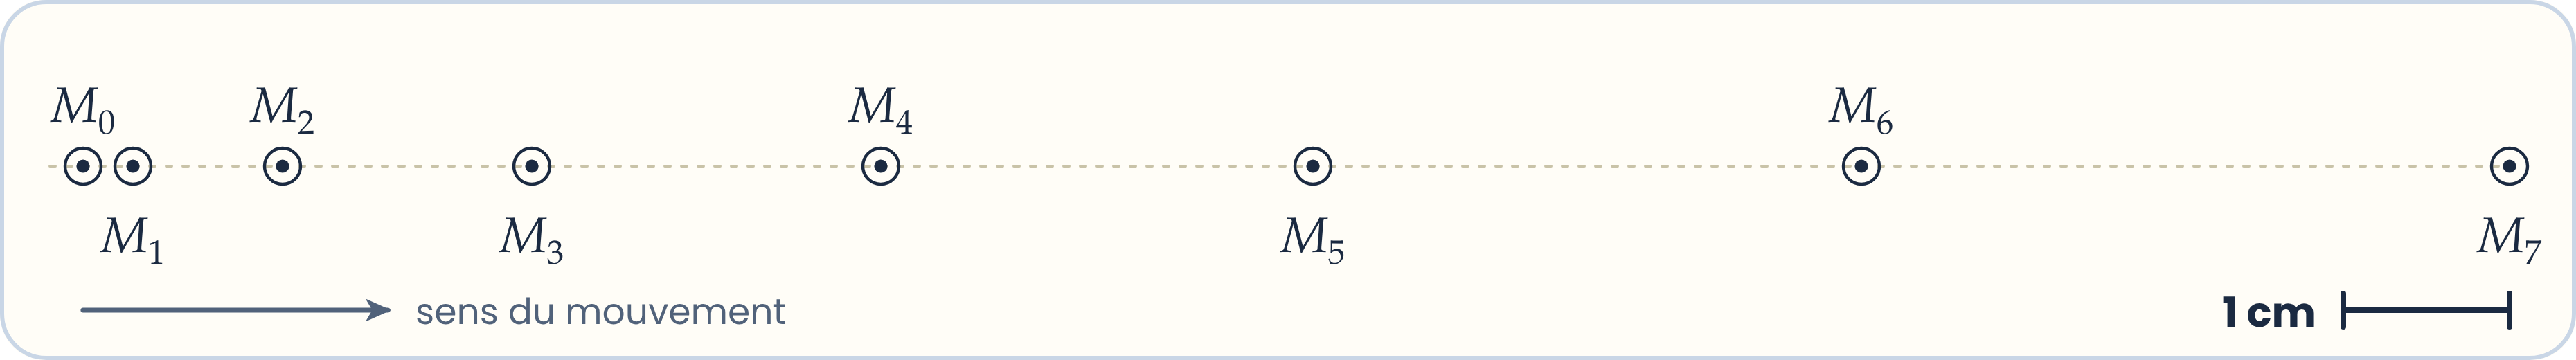
\includegraphics[width=15.5cm]{doc8_enregistrement}\par\vspace{.5mm}
{\sffamily\scriptsize\docbadge{8}\enspace\color{cInk2}Enregistrement à l’échelle 1 (positions du centre d’inertie) — \textbf{imprimer à 100 \%}}
\end{minipage}\par}
\vspace{.6mm}
\begin{enumerate}
  \item \kw{Calculer.} Chute libre (doc 6) : calculer en chaque point $A_i$ la vitesse $V_i = \dfrac{d}{\Delta t}$, l’énergie cinétique $E_{\mathrm{C}i}$ et le travail du poids $W_{A_1\to A_i}(\vect P) = m\cdot g\cdot(h_i - h_1)$. Présenter les résultats dans un tableau.
  \item \kw{Analyser.} Tracer la courbe $\Ec = f\big(W(\vect P)\big)$. Quelle est sa forme ? Interpréter son ordonnée à l’origine, calculer son coefficient directeur et en déduire une relation entre $\Delta\Ec = E_{\mathrm{C}i} - E_{\mathrm{C}1}$ et $W(\vect P)$.
  \item \kw{Inventorier.} Plan incliné (docs 7 et 8) : faire le bilan des forces qui s’exercent sur le mobile. Exprimer la somme de leurs travaux entre $M_1$ et $M_i$ en fonction de $m$, $g$, $D_i$ et $\alpha$.
  \item \kw{Calculer.} Exprimer la vitesse $V_i$ en fonction de $d_i$ et $\tau$. Calculer $E_{\mathrm{C}i}$ et $W_{M_1\to M_i}(\vect P)$ pour les points $M_1$ à $M_6$.
  \item \kw{Généraliser.} La courbe $\Ec = f\big(W(\vect P)\big)$ du mobile est une droite. Écrire son équation et en déduire la relation générale entre $\Delta\Ec$ et la somme des travaux des forces extérieures.
\end{enumerate}

% =====================================================================
\sep{4}
\begin{minipage}[t]{0.66\linewidth}\vspace{0pt}\RaggedRight
\textbf{Doc 9.} Un volant de moment d’inertie $J_\Delta$ tourne autour d’un axe fixe $(\Delta)$, dans un référentiel galiléen. Sous l’action de forces extérieures (dont certaines ont un moment non nul par rapport à l’axe), sa vitesse angulaire passe de $\omega_1$ à l’instant $t_1$ à $\omega_2$ à l’instant $t_2$. Chaque élément de matière du volant subit une variation d’énergie cinétique égale au travail des forces qui s’exercent sur lui. En additionnant ces relations pour tous les éléments du solide indéformable, on obtient une relation pour le solide entier, valable même si les forces ou leurs moments ne sont pas constants.\par\vspace{.6mm}
\begin{enumerate}
  \item \kw{Écrire.} Écrire le théorème de l’énergie cinétique pour le volant du doc 9, dont la vitesse angulaire passe de $\omega_1$ à $\omega_2$.
  \item \kw{Énoncer.} Énoncer le théorème de l’énergie cinétique valable pour un solide en translation ou en rotation autour d’un axe fixe. Reste-t-il valable si les forces ou leurs moments varient ?
  \item \kw{Ordonner.} Quelles étapes faut-il suivre pour appliquer ce théorème à un système mécanique ?
\end{enumerate}
\end{minipage}\hfill
\doc{0.3\linewidth}{9}{Volant entraîné par un moteur}{doc9_volant}
\end{document}
